\subsection{Programmable Privacy}

Programmability The privacy platform has two main features (1)It supports private 
transactions, not only private transactions. Similar to Zcash \cite{website:Zcash}, users can still 
choose the transaction type, public transaction or private transaction independently; 
(2)Support Programmability, you can deploy any smart contract, public contract or 
private contract, depending on the needs of the project party. Compared with Specific 
Privacy, the main difference is the logic of state transition in Note, from specific 
calculation to arbitrary calculation logic. Figure \ref{fig:Difference between Specific Privacy and Programmable Privacy} simply shows the difference 
between the two.
\begin{figure}[!ht]
    \centering
    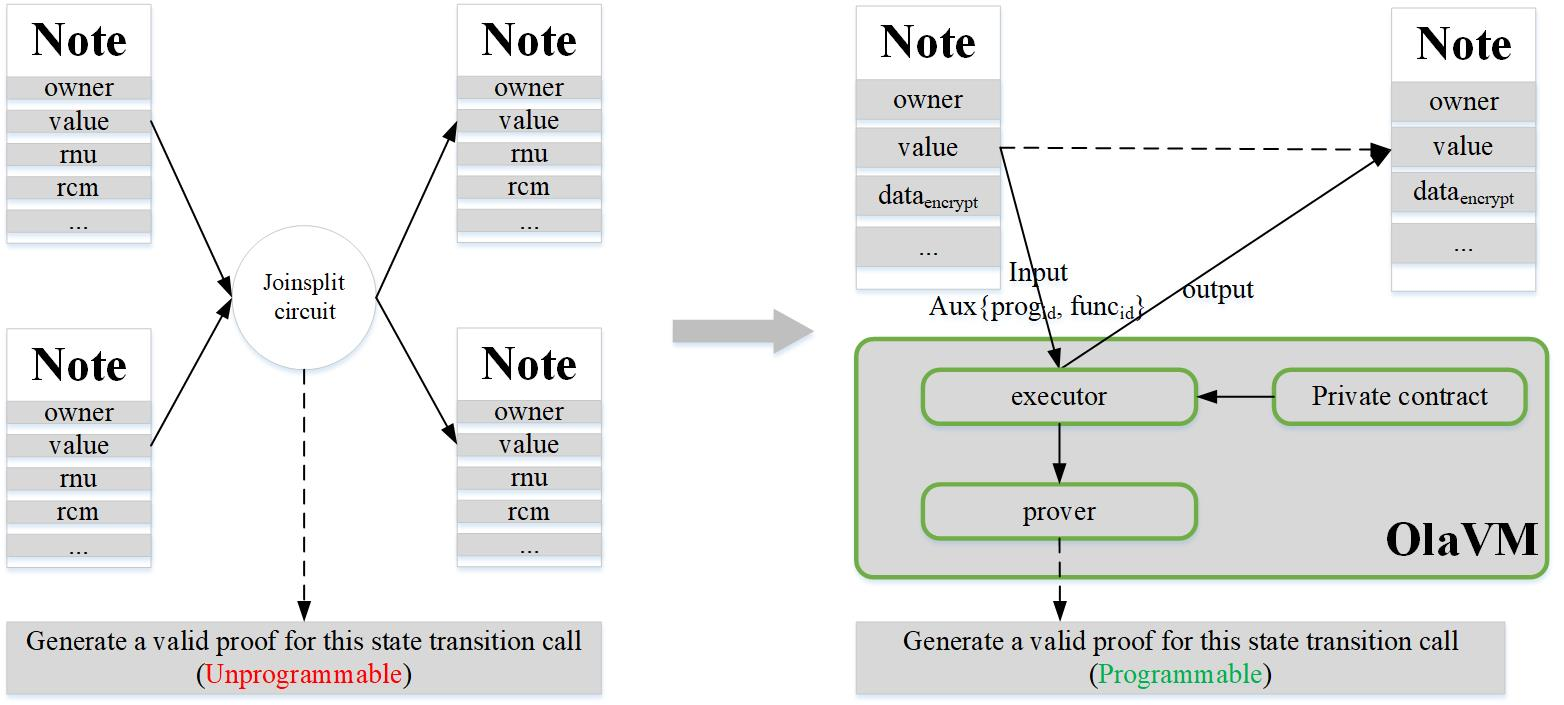
\includegraphics[width=0.8\textwidth]{Difference between Specific Privacy and Programmable Privacy.jpg}
    \caption{Difference between Specific Privacy and Programmable Privacy}
    \label{fig:Difference between Specific Privacy and Programmable Privacy}
\end{figure}

The current projects focusing on programmable privacy are Aleo \cite{website:Aleo} and Aztec \cite{website:Aztec}. Aleo \cite{website:Aleo} is a 
privacy public chain, from BTC \cite{website:BTC} to Ethereum \cite{website:Ethereum} to Zcash \cite{website:Zcash} to Aleo \cite{website:Aleo}. It makes up for 
the fact that programmability and privacy cannot coexist at the Layer1 level. 
It has reached the testnet stage and supports developers to deploy privacy contracts; 
Aztec \cite{website:Aztec} focuses on doing Layer2 programmable privacy for Ethereum \cite{website:Ethereum} , a project 
called Aztec3 \cite{website:Aztec3}, is still in development.